 %%%%%%%%%%%%%%%%%%%%%%%%%%%%%%%%%%%%%%%%%%%%%%%%%%%%%%%%%%%%%%%%%%%%%%%%%%%%%
%	e-Yantra, IIT-Bombay

%	Document Author: Akshit Gandhi
%	Date: 17-June,2016
%	Last Editted by: Akshit
%   Date Last updated: 17-06-2016 

%%%%%%%%%%%%%%%%%%%%%%%%%%%%%%%%%%%%%%%%%%%%%%%%%%%%%%%%%%%%%%%%%%%%%%%%%%%%%

\documentclass[11pt,a4paper]{article}
\usepackage{float}
\usepackage{graphicx}
\usepackage{hyperref}
\usepackage{float}
\title{Interfacing Raspberry-pi with APM flight controller}
\author{Akshit Gandhi \\ Keyur Rakholiya}

\date{\today}

\begin{document}
	\maketitle
	\newpage
	\tableofcontents
	\newpage
	\section{Objective}
	Topic: Interfacing Raspberry-pi with APM(ARDUPILOT) flight controller
			APM is a flight controller which performs the stabilization of quadcopter by varying the signal to the motors based upon Radio control input. It has different flight modes which we can set from remote. It also supports different sensors like GPS ,Sonar etc.
		In this tutorial we will learn to how to setup a communication between the 
		 and APM flight controller, so that we can run/write our python scripts on R-PI and execute them on our drone. We will be going into details of each step.
	\section{Prerequisites}
	 It's better if you first go through the official documentation on ardupilot's website on connecting R-PI		 with APM.\textbf{[1]}, it will be beneficial also for this tutorial and also for later tutorials.
	\section{Hardware Requirement}
	 Drone or Quadcopter, Raspberry pi, telemetry port connector for connecting APM to RPI and few jumpers(M-F).
	\section{Procedure}
	This tutorial explains how to connect and configure a Raspberry Pi (RPi) so that it is able to communicate with a APM flight controller using the MAVLink protocol\textbf{[2]} over a serial connection
	 \begin{figure}[H]
	 	\centering
		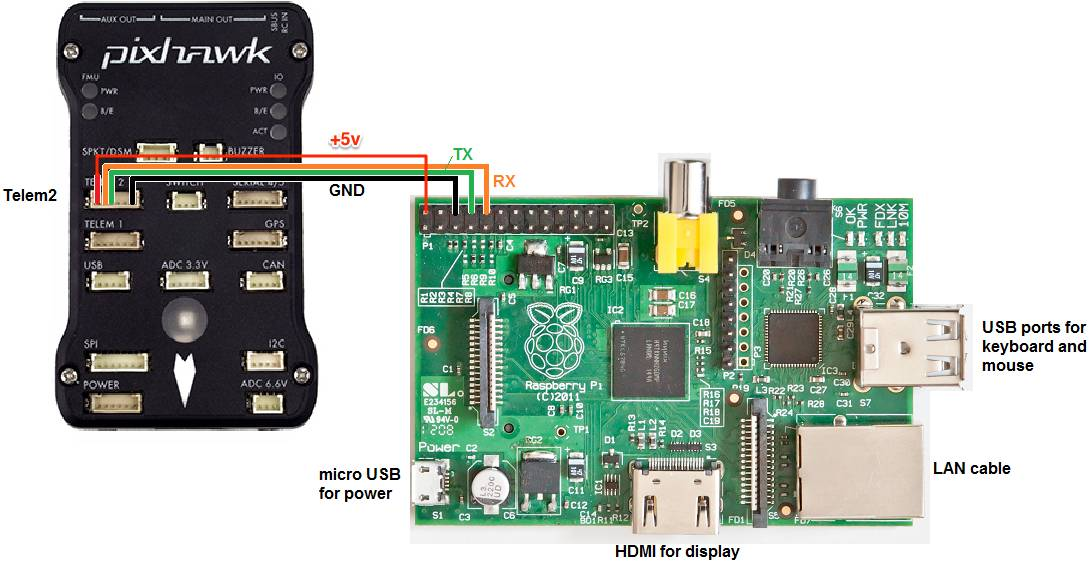
\includegraphics[scale=0.35]{wiring}
	 	\caption{Connection diagram.}
\end{figure}
	\paragraph{•} The picture shown above is for pixhawk controller but the same connection works for APM also.
	 \subsection{Connecting to RPi with an SSH/Telnet client}
	 \textbf{NOTE:} These steps assume that you have already set-up your RPi so that it is running Raspbian.

To avoid the requirement to plug a keyboard, mouse and HDMI screen into your RPi it is convenient to be able to connect from your Desktop/Laptop computer to your RPi using an SSH/Telnet client such as PuTTY.
	 \begin{itemize}
	 	\item Connect the RPi to your local network by one of the following methods:
			\begin{itemize}
				\item Connecting an Ethernet LAN cable from the RPi board to your Ethernet router, or
				\item Use a USB dongle to connect your RPi to the local wireless network, or
				\item Connect the Ethernet LAN cable between the RPi and your desktop/laptop computer. Open the control panel’s Network and Sharing Center, click on the network connection through which your desktop/laptop is connected to the internet, select properties and then in the sharing tab, select “Allow other networks to connect through this computer’s Internet connection”
\end{itemize}
	\item Determine the RPi’s IP address:
	\begin{itemize}
		\item If you have access to the RPi’s terminal screen (i.e.you have a screen, keyboard, mouse connected) you can use the /sbin/ifconfig command.
			\begin{figure}[H]
				\centering
				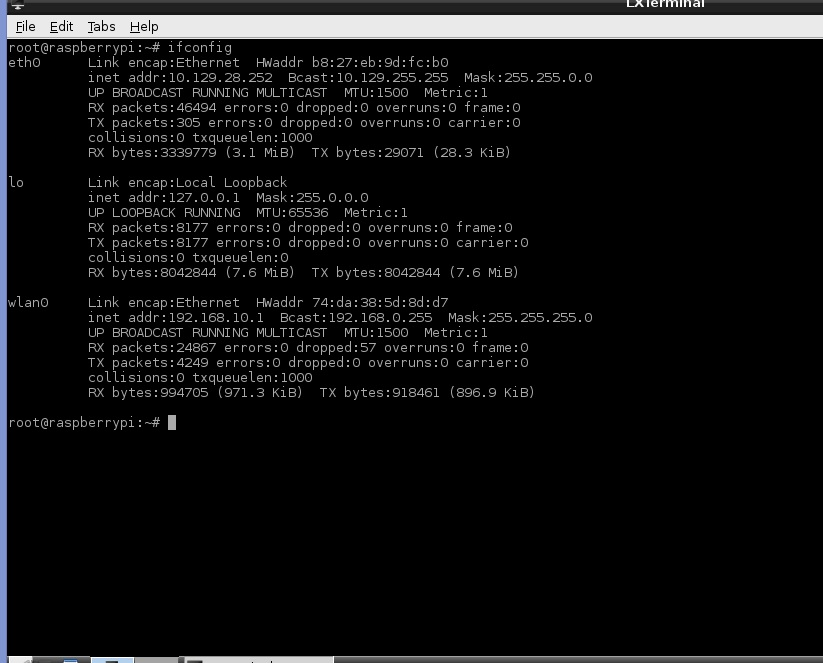
\includegraphics[scale=0.37]{ip}
				\caption{ip address on terminal.}
			\end{figure}
		\item If your Ethernet router has a web interface it may show you the IP address of all connected devices
	\end{itemize}	\item Connect with Putty:
		\begin{figure}[H]
	 	\centering
		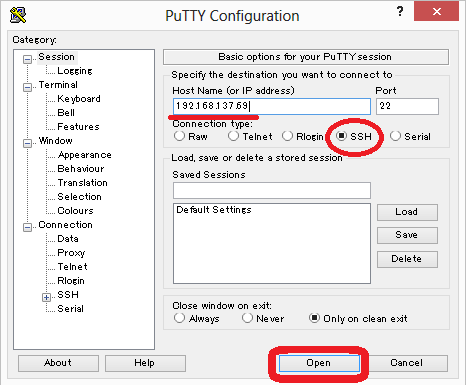
\includegraphics[scale=0.37]{putty}
	 	\caption{Connect screen with Putty.}
\end{figure}
	If all goes well you should be presented with the regular login prompt to which you can enter the username/password which defaults to pi/raspberry
	 \end{itemize}
	 \subsection{Install the required packages on the Raspberry Pi}
	 Log into the RPi board (default username password is pi/raspberry) and check that its connection to the internet is working. If there's some problem then troubleshooting guide can be found on the documentation site \url{http://ardupilot.org/dev/docs/raspberry-pi-via-mavlink.html}
	 \paragraph{After the internet connection is confirmed to be working install these packages:}
	 \begin{itemize}
	 	\item sudo apt-get update
	 	\item sudo apt-get install screen python-wxgtk2.8 python-matplotlib python-opencv python-pip python-numpy python-dev libxml2-dev libxslt-dev
	 	\item sudo pip install pymavlink
	 	\item sudo pip install mavproxy
	 \end{itemize}
	 \subsection{Disable the OS control of the serial port}
	 Use the Raspberry Pi configuration utility for this.
		\paragraph{}Type:
			\begin{itemize}
				\item sudo raspi-config
				\item And in the utility, select 								“Advanced Options”:
				\begin{figure}[H]
	 	\centering
		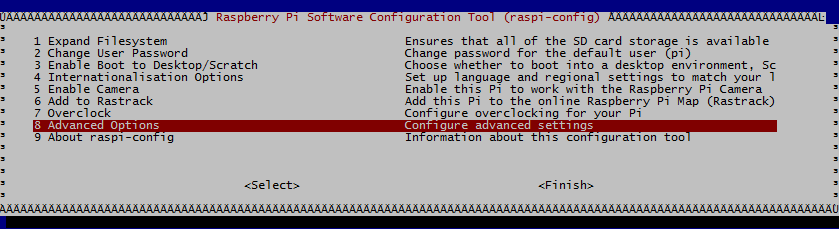
\includegraphics[scale=0.37]{adv1}
	 	\caption{RasPiConfiguration Utility: Serial Settings: Advanced Options.}
\end{figure}
		\begin{itemize}
			\item And then “Serial” to disable OS use of the serial connection:
			\begin{figure}[H]
	 	\centering
		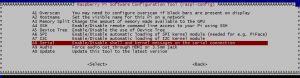
\includegraphics[scale=0.85]{adv2}
\end{figure}
		\end{itemize}
Reboot the Raspberry Pi when you are done.
			\end{itemize}
			\subsection{Testing the connection}
			To test the RPi and APM are able to communicate with each other first ensure the RPi and APM are powered, then in a console on the RPi type:
			\begin{itemize}
				\item sudo -s
				\item mavproxy.py --master=/dev/ttyAMA0 --baudrate 57600 --aircraft MyCopter
				
				raspberry pi's default port is connected with console input/output. so use this port we have to disable it first. now we have connected our device via UART port ot R-Pi. so "/dev/ttyAMA0" is a port for serial communication between R-pi and APM. 
				
				You configure BaudRate as bits per second. The transferred bits include the start bit, the data bits, the parity bit (if used), and the stop bits. However, only the data bits are stored.
				
				The baud rate is the rate at which information is transferred in a communication channel. In the serial port context, "9600 baud" means that the serial port is capable of transferring a maximum of 9600 bits per second. If the information unit is one baud (one bit), the bit rate and the baud rate are identical. If one baud is given as 10 bits, (for example, eight data bits plus two framing bits), the bit rate is still 9600 but the baud rate is 9600/10, or 960. You always configure BaudRate as bits per second. Therefore, in the previous example, set BaudRate to 9600.
				
				 
				Note: In the above command it's MyCopter and My-Copter
				\item Once MAVProxy has started you should be able to type in the following command to display the \texttt{ARMING\_CHECK} parameters value
				\begin{itemize}
					\item param show \texttt{ARMING\_CHECK}
					\item param set \texttt{ARMING\_CHECK} 0
					\item arm throttle
					\begin{itemize}
			\item And then “Serial” to disable OS use of the serial connection:
			\begin{figure}[H]
	 	\centering
		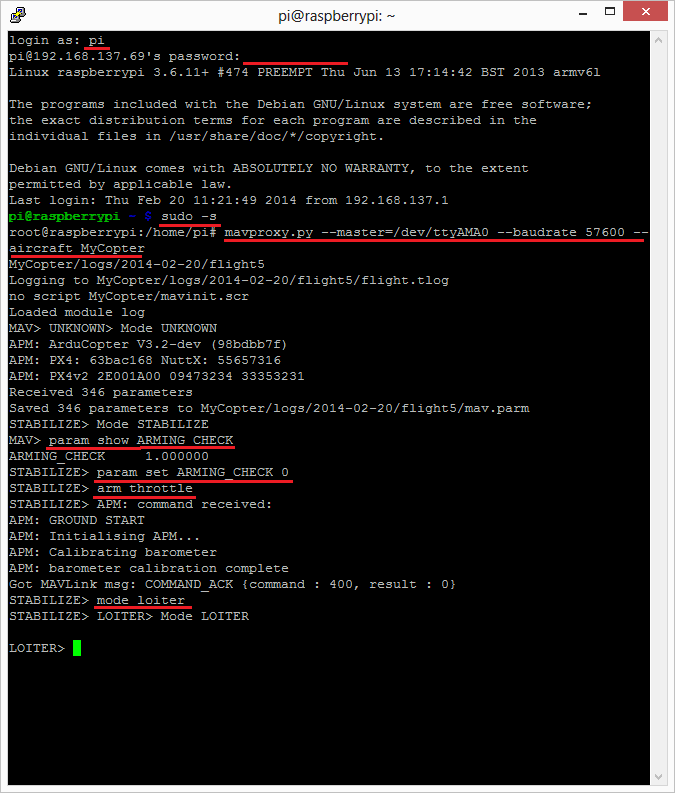
\includegraphics[scale=0.6]{connect}
		\caption{Terminal screen.}
\end{figure}
	\textbf{NOTE:} If you get an error about not being able to find log files or if this example otherwise doesn’t run properly, make sure that you haven’t accidentally assigned these files to another username, such as Root.
	\paragraph{•}Entering the following at the Linux command line will ensure that all files belong to the standard Pi login account:
	\item sudo chown -R pi /home/pi
		\end{itemize}
				\end{itemize}
				
			\end{itemize}
			\subsection{Configure MAVProxy to always run}
				To setup MAVProxy to start whenever the RPi is restarted open a terminal window and edit the /etc/rc.local file, adding the following lines just before the final “exit 0” line: 
				\begin{figure}[H]
	 	\centering
		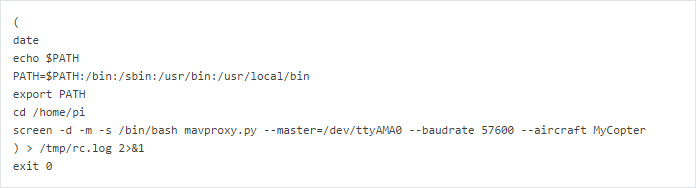
\includegraphics[scale=0.75]{command}
		
\end{figure}
\paragraph{To open /etc/rc.local file type in sudo nano /etc/rc.local and type the code below and save it in the file}
\paragraph{}If you wish to connect to the MAVProxy application that has been automatically started you can log into the RPi and type: sudo screen -x
\paragraph{•}It is also worth noting that MAVProxy can do a lot more than just provide access to your APM. By writing python extension modules for MAVProxy you can add sophisticated autonomous behaviour to your vehicle. A MAVProxy module has access to all of the sensor information that your APM has, and can control all aspects of the flight.
	\section{References}
	\paragraph{•}
	\textbf{[1]}\url{http://ardupilot.org/dev/docs/raspberry-pi-via-mavlink.html}
	\textbf{[2]}\url{http://qgroundcontrol.org/mavlink/start}
	\url{http://ardupilot.org/dev/docs/raspberry-pi-via-mavlink.html}
		
	\paragraph{Everything mentioned above bit by bit is from the official documentation.}
	
\end{document}



